\documentclass[12pt,fleqn]{article}\usepackage{../common}
\begin{document}
Ders 25

Gectigimiz birkac haftada duzlemde cift entegral, duzlemde cizgi entegrali
hesaplarini gorduk. Artik bu dersten baslayarak benzer teknikleri
gorecegiz, ama bu teknikleri 3 boyutlu uzayda gorecegiz. Yani uzayda uclu
entegral, uzayda akis (flux), uzayda is (work), uzaklasim (divergence),
curl hesaplari gibi. Bu yeni hesaplar aslinda simdiye kadar gorduklerimizin
ek bir eksen eklenmis hali, bazi farkliliklar var, ama kavramsal olarak
ayni seyler. O yuzden tavsiyem eger duzlemde yapilan hesaplari tam
anlamadiysaniz, geri donup bu konulari bir daha gozden gecirmeniz. 

Uclu Entegral (Triple Entegrals)

Eger 3 boyutta size bir kutle verirsem, 

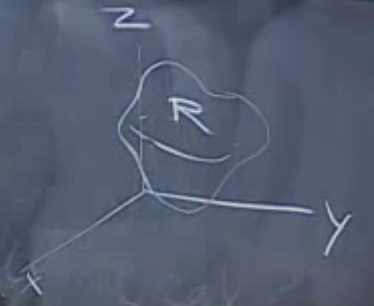
\includegraphics[height=3cm]{25_1.png}

bu alan uzerinden uclu entegral alabilirim, 

\[ \int \int \int _R f dV \]

$V$, hacim (volume) anlaminda, yani $dV$ ile $R$ kutlesinin icindeki sonsuz
ufakliktaki hacimleri dusunuyoruz, ve onlari topluyoruz. $dV$ buyuklugu,
$dx,dy,dz$ sonsuz ufakliklara tekabul eder, tabii siralama her turlu
sekilde olabilir.

Eger ikili olarak ozyineli entegralleri nasil hazirlayacagimizi biliyorsak,
uclu entegraller de buna benziyor. Iki onemli kavram var, biri entegrasyon
alani, digeri entegre edilen fonksiyon. Fonksiyon tabii ki entegrasyon
hesabini tamamlarken onemli, ama daha zor olan adim entegrali
hazirlayabilmek. 0 yuzden bugun hazirlik asamasina odaklanacagim,
kullanacagim fonksiyonlar basit seler olacaklar. 

Ornek 

Bolge $x = x^2 + y^2$ ve $z = 4 - y^2 - x^2$ arasindaki bolge. Diyelim ki
bu bolgenin sadece hacmini hesaplamak istiyorum, yani $f = 1$ yeterli. 

\[ \int \int \int 1 \ dV \]

Hatirlarsak alan icin cift entegrallerde $1 \ dA$ kullanmistik, benzer
numara. 












\end{document}
